\chapter{La relative diversité de la représentation des dommages}
\label{chapter:litrev}
\newrefsegment

\PEEL{Les manières de représenter les dommages du changement climatique varient selon leur niveau de désaggrégation, le type de modèle utilisé (simulation / optimisation), leur calibration et les phénomènes qu'elles prennent en compte. }{Nordhaus et Stern se disputent sur la valeur du taux d'actualisation (avec pourtant les mêmes modèles). Le SCC est calculé aux US alors que les dommages ne sont pas pris en compte dans les modèles de l'IIASA database. Il y a une forte utilisation des indicateurs économiques. }{Ces différents duels montrent la diversité de choix possibles offerts aux modélisateur.ices.}{Répondre à ces questions est un choix important, qui dépasse le pure cadre technique pour rejoindre la dimension éthique.}


\chapterabstract{Les fonctions de dommage permettent de modéliser les impacts du changement climatique sur d'autres parties du modèle. Elles peuvent varient par leur existence, forme, calibration ou par les paramètres ou secteurs qu'elles prennent en compte. Pourtant, un changement dans ces fonctions peut radicalement faire changer le fonctionnement d'un modèle, et ainsi les résultats et les conclusions qu'on en tire. Cette partie s'intéresse donc aux différentes fonctions de dommage qui existent dans la littérature.}

%%Accroche
Les modèles intégrés sont ainsi derrière de nombreuses publications qui informent le débat public : rapports du GIEC, Stern Review, revue du coût social du carbone. Ils ont donc un rôle de premier plan dans la prise de décisions sur les questions climatiques, sur les options qu'ils estiment possibles ainsi que sur les conséquences anticipées de telle ou telle action. Un élément clé de cette modélisation est la prise en compte des impacts climatiques. 


%%Définition des termes

%%Rappel du sujet
Les différentes formes de fonction de dommage dans les modèles intégrés

%%Problématique
Quelles sont les fonctions de dommages utilisées dans les modèles intégrés ? Et, plus précisement, quels modèles utilisent des fonctions de dommage ? Quels phénomènes sont représentés ? Quelles variables entrent en compte, et comment sont-elles paramétrisées ? 

%% Annonce du plan
Dans une première partie, nous détaillerons la méthodologie utilisée pour obtenir la base de donnée des fonctions de dommage. Dans une seconde partie, nous la décrirons avec différentes statistiques descriptives. Enfin, nous aborderons trois points critiques des fonctions de dommage : leur forme; leurs paramètres; et la calibration. 

\begin{methodbox}[Revue de la littérature]
Pour obtenir une base de données des différentes fonctions de dommage, nous avons cherché à fusionner plusieurs sources de données. D'abord, l'IAM Consortium publie sur son site internet les documentations de nombreux modèles intégrés, sous la forme d'un wiki. Ces fiches sont rédigées par les équipes des modèles - ce qui permet d'avoir une source primaire sur les informations concernant les modèles - mais sont souvent incomplètes. En revanches, des "cartes", qui détaillent les principales caractéristiques de chaque modèle, sont également disponibles. Ce sont principalement celles-ci qui sont utilisées dans la base de données. Une autre source de données est le fichier des scénarios utilisés par le GIEC. Celui-ci permet d'avoir des informations sur chacun des scénarios soumis pour l'AR6, et d'avoir accès à de nombreuses informations : modèle utilisé, vetted ou non, impacts climatiques pris en compte ou non. A ces différentes sources, on ajoute manuellement des modèles, basée sur une lecture aléatoire de la littérature. Ils comprennenent notablement les modèles utilisés par l'agence interagence du coût social du carbone, ceux cités par Souffron et Jacques, ceux utilisés par les SSP, ainsi que d'autres modèles intégrés trouvés par littérature interposée. 
Le monde de la modélisation est très vaste, les modèles souvent compliqués à comprendre et parfois peu transparents. Ainsi, il a toujours été préféré de se baser sur des sources explicites. Bien qu'un véritable effort pour chercher à avoir une vision sur le plus de modèles possibles, cette étude ne peut pas être considérée comme un recensement exhaustif des modèles intégrés ni de leurs fonctions de dommage. \\ \gls{latex}

Une fois cette première liste de modèles obtenue, un premier tri est effectué entre ceux qui intègrent une fonction de dommage et ceux qui n'en intégrent pas. On considére ici les fonctions de dommages explicitement définies telles quelles, bien que d'autres fonctions puissent in fine avoir un comportement similaire. Ainsi, pour certaines, on a une connaissance explicite : par exemple, les fiches de l'IAMC comportent une case sur les impacts modélisés. Pour les autres, on considère qu'elles n'ont pas de fonction de dommage si les termes "damage function" ou "damage" ne sont pas présents dans leur documentation ou les publications associées, et s'il n'est pas fait mention de fonctions de dommage dans d'autres sources. \\

Pour chaque modèle incluant des fonctions de dommage, on cherche dans sa documentation la description de ces fonctions de dommage. La plupart du temps, celle-ci comporte une équation et les variables associées. Un script Chat-GPT est alors utilisé sur la partie du document qui est décrit la fonction de dommage. Celui-ci interprète et met en forme (sous la forme d'un tableau CSV) toutes les variables présentes dans cette fonction. Elles sont alors contrôlées visuellement. Cette étape est repétée pour chaque fonction de dommage. Une fois les variables de chaque fonction de dommage d'un modèle identifiées, ce fichier est téléversé dans la base de données, à l'aide du logiciel Airtable, dans la table 'Variable'. \\

Une fois les variables insérées dans leur table, les fonctions de dommage sont incluses dans la table 'Damage functions'. Chaque fonction est assortie à un nom, soit celui-donné dans la publication, soit choisi selon le contexte. Sont également ajoutés le nom du modèle, le numéro de l'équation, l'annotation zotero et le DOI de la publication, afin de pouvoir retrouver rapidement la fonction de dommage. Sont alors ajoutés d'une part les variables qui viennent en entrées de l'équation, et la variable qui sur laquelle l'équation agit. \\

Enfin, une autre table est ajoutée : celle des risques identifiés par le GIEC. Ceux-ci sont issus du rapport de synthèse de l'AR6, et la classification est faite par l'auteur. Lorsqu'une fonction de dommage décrit un des risques identifiés par le GIEC, elle se voit liée à celui-ci. 



\end{methodbox}

\begin{figure}
    \centering
    %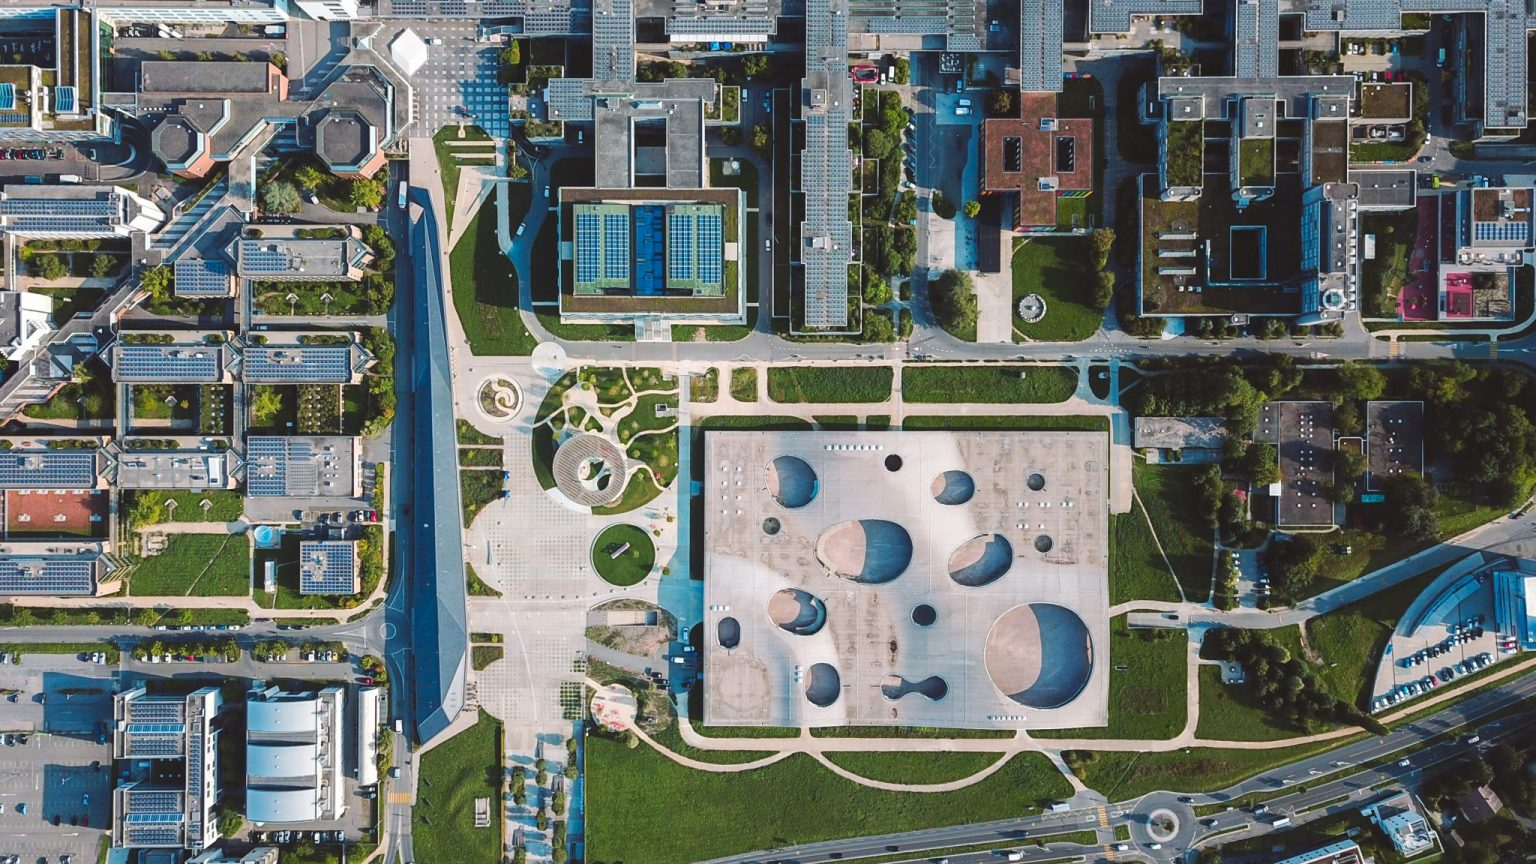
\includegraphics{figures/campus.jpg}
    \legende{Processus de sélection des modèles.}{Les modèles sont sélectionnées selon plusieurs critères : présence dans une des bases de données (GIEC, SCC, SSP, IAMC) ou dans une review. Ils sont ensuite comparés selon leurs caractéristiques.}
    \label{fig:méthodo-litrev}
\end{figure}

\section{Tour d'horizon des modèles et de leurs fonctions de dommage}

Les modèles intégrés sont très variés. Ils ont des histoires différentes (issus de l'énergie, de l'économie ou du climat), des perspectives différentes (en particulier entre les États-Unis ou l'Union européenne), des questions différentes, des choix de modélisation différents (simulation ou optimisation). 

Revue de la littérature se classe en 3 catégories : la construction des IAMs, la comparaison des résultats des IAMs, les articles iam par iam

\subsection{Une littérature composée d'article par modèle ou de méta-analyses}

La littérature existante s'articule autour de trois axes. D'abord, il y a une abondante littérature autour des modèles. En effet, chaque modèle fait l'objet de nombreuses publications pour en présenter la structure, puis pour en donner les résultats. Il y a par ailleurs de nombreuses ressources appartenant à la littérature grise : des blogs, du code source, des rapports aux commanditaires, des modèles, etc. Ensuite, il y a des méta-analyses qui comparent les résultats des modèles; enfin, tout un pan de la littérature s'intéresse à la structure même des modèles, à travers des comparaisons entre modèles. 

\subsubsection{Documentation et résultats de chaque modèle}

\paragraph{Les modèles sont accompagnés d'analyses}

La principale source d'information que l'on a sur les modèles est les publications scientifiques qui en présentent les résultats.
Il s'agit de publications qui démontrent quelque chose ou répondent à une question (voir, par exemple, \cite{int_panis_externe_2000, dafermos_how_2021, baumstark_remind21_2021, dafermos_stock-flow-fund_2017, cherp_global_2016, burke_global_2015}). Le modèle et/ou la fonction de dommage y sont peu décrits (au plus une équation sans paramétrisation), souvent dans la section méthodologie. Ces articles sont intéressants car ils permettent de comprendre la finalité des modèles, les conditions pour lesquelles ils ont été conçus. En revanche, ils ne permettent pas à eux seuls de reproduire l'analyse ou de la modifier. 


\paragraph{Le niveau de documentation et d'ouverture varie considérablement}

Une autre source de documentation est la littérature grise qui accompagne les publications scientifiques. On en trouve des formes très variées, telles que des rapports (voir \cite{medeas_guiding_2019, asbjorn_aaheim_grace_2018, european_commission_ginfors-e_2022, european_commission_gem-e3_2013, nordhaus_dice_2013}), des \emph{working papers} (voir par exemple \cite{dafermos_stock-flow-fund_2017, giraud_coping_2016, calvin_gcam_2019, bosetti_witch_2006, ghersi_imaclim-p_2014}), des blogs (voir par exemple \cite{tol}

\paragraph{}

\subsubsection{Sur les résultats des IAMs}





Meta analyse des estimations du niveau du changement climatique
\cite{howard_few_2017} => 

\cite{gillingham_modeling_2018} gillingham => peut être à mettre dans la partie \ref{chapter:modelisation} ?

\cite{keppo_exploring_2021} => grosse revue de littérature sur les IAMs

\cite{harmsen_integrated_2021} => évaluation des IAMs à travers une méthodologie précise




\subsubsection{Sur la structure des IAMs }

\paragraph{Il existe des fonctions de dommage, mais sous des modèles semblables entre eux et orthodoxes.}

Dans une importante revue de littérature sur l'évaluation des dommages climatiques par les modèles intégrés, \cite{diaz_quantifying_2017} passe en revue les caractéristiques et contraintes liées aux fonctions de dommages. Elle inspecte en particulier DICE, FUND et PAGE, qui sont trois modèles conçus spécifiquement pour évaluer monétairement les impacts. Elle formule de nombreuses critiques : l'extrapolation à de hautes températures ou à d'autres régions, le choix des impacts représentés, l'absence d'interaction inter-régionales ou temporelles, l'absence de représentation de l'adaptation, des données scientifiques datées, la représentation lacunaire de l'incertitude, et d'autres encore. 

Cet article a servi de réference à la suite de ce travail. Néanmoins, les modèles représentés sont similaires, avec des objectifs similaires et produits par des communautés scientifiques proches. Or, la plupart des critiques faites par Diaz sont liées à des méthodes de modélisation ou  à des hypothèses générales. Pour comparer ces modèles et défier ces hypothèses, il faut sortir de cette communauté.  \\


Nous nous intéressons donc à d'autres revues de littératures, plus large, mais permettant d'avoir un plus large panel de modèles. 

\paragraph{Chercher des modèles plus divers permet de répondre à certaines des critiques}


Par exemple, \cite{souffron_successful_2024} cherchent à explorer la diversité des modèles, et montrent qu'un plus large panel de modèles permet de mieux guider les politiques publiques. Ils montrent que les modèles orthodoxes sont particulièrement limités. Ils présentent ensuite des modèles alternatifs, mettant en avant les atouts et contraintes de chacun. Enfin, ils émettent des recommandations de caractéristiques que pourraient avoir des modèles idéaux, notamment le fait d'avoir des fonctions de dommage. 






\cite{souffron_successful_2024} => présente plein de modèles et les commente. Pas vraiment une revue de littérature sur les damage functions mais plus général, permet de bien se repérer dans la littérature + grosse emphase sur les modèles hétérodoxes

\cite{review of information on models}  Une revue des différents modèles 

\paragraph{D'autres revues comparent des hypothèses plus varéies dans les modèles}

\cite{krey_looking_2019} => comparaison des hypohtèses technologiques des modèles

Sur les types de modèles : 
\cite{mercure_modelling_2019} => présente les principales différences entre les modèles de simulation et d'optimisation, et montre que c'est aussi une différence paradigmatique. 

\paragraph{La place particulière de l'IAMC}


Il y a une multitude de ressources liées à la modélisation des dommages dans les modèles intégrés. Il n'existe pourtant pas de plateforme unique permettant de recenser toutes les formes de fonctions de dommage, leurs effets, atouts et contraintes. 

\section{Méthode : construction de la base de données}



\subsection{Les principaux modèles}

On présente ici rapidement des modèles, leurs caractéristiques générales et la forme de leur fonction de dommage. Il s'agit surtout de montrer la diversité des approches de modélisation, et non d'avoir un recensement systématique. Les lecteurs plus curieux trouveront plus de caractéristiques en suivant le lien. \blog{https://damage-functions-modeling.readthedocs.io/en/latest/1_introduction/functions.html}

\subsubsection{DICE}

DICE veut dire \emph{Dynamic Integrated model of Climate and the  Economy} et constitue une des premières tentatives de modéliser les relations entre l'économie et le climat. Il comporte une fonction de dommage, extrêmement simplifiée. 

\begin{equation}
\begin{array}{ll}
     \displaystyle  \Delta  & = \psi_{1}T_{AT}(t) + \psi_{2}[T_{AT}(t)]^{2} \\
    & = [0.0]T_{AT}(t) + [0.003467][T_{AT}(t)]^{2}
\end{array}
\label{eq:df_dice2023}
\end{equation}

Avec : 
\begin{itemize}
    \item $\Delta$ le niveau de dommage, en pourcentage du PIB
    \item $T_{AT}$ le niveau de réchauffement climatique, en degré celsius
    \item $\psi_1, \psi_2$ des paramètres permettant de calibrer la fonction
\end{itemize}

Celle-ci est calibrée de manière à correspondre à des estimations issues du sixième rapport du GIEC et d'autres sources. Ils donnent un dommage de 1.62 \% du PIB pour un réchauffement de 3$\textdegree$C par rapport au niveau préindustriel \cite{barrage_policies_2023, nordhaus_dice_2013}. 

\subsubsection{FUND} 

A l'inverse, FUND présente un niveau de désagrégation assez avancé. Il y a de nombreuses fonctions de dommage, qui sont utilisées les unes dans les autres. Leur forme générale est d'obtenir un niveau de dommage à partir d'une élasticité entre un phénomène et un autre. \\

Par exemple, l'impact du changement climatique sur l'agriculture est construit par la somme de trois canaux : d'une part, l'impact du niveau de changement climatique; d'autre part, la vitesse de ce changement (représenté en \ref{eq:fund_A2}); enfin, l'augmentation de la fertilisation des plantes. 

\begin{equation}
    A_{t,r}^{r}=\alpha_{r}\left(\frac{\Delta T_{t}}{0.04}\right)^{\beta}+\left(1-\frac{1}{\rho}\right)A_{t-1,r}^{r}
    \label{eq:fund_A2}
\end{equation}

D'autres impacts sont aussi représentés, tels que l'impact du niveau des eaux sur le littoral, les écosystèmes, les dommages liés aux cyclones tropicaux et extra-tropicaux, etc., et ce par différents biais : des dommages directs (monétaires), et la monétarisation de perte de vie ou de perte de temps de vie. 

On peut citer par exemple cette fonction (HV) qui permet d'estimer le nombre de morts additionnelles issus des maladies transmissibles  :  
\begin{equation}
    D_{t,r}^{\nu}=D_{1990,r}^{\nu}Q_{r}^{\nu}\left(T_{t}-T_{1990}\right)^{\beta}\left(\frac{y_{t,r}}{y_{1990,r}}\right)^{\gamma}
    \label{eq:fund_HV}
\end{equation}
avec : 
\begin{itemize}
    \item $D^v_{t,r}$ est l'augmentation de la mortalité due à la maladie $v$, dans la région $r$ à l'instant $t$ 
    \item $D^v_{1990,r}$ la mortalité due à la maladie $v$ dans la région $r$ en 1990
    \item $t$ l'année
    \item $r$ la région
    \item $v$ la maladie
    \item $\alpha$ un paramètre issu de dires d'expert (\emph{"expert guess"})
    \item $y_{t,r}$ le revenu par habitant dans la région $r$ à l'instant $t$ 
    \item $T_t$ la température moyenne à l'instant $t$
    \item $\beta = 1.0$ un paramètre représentant la linéarité de la mortalité selon la température (c'est-à-dire la manière dont la mortalité évolue selon la température)
    \item $\gamma = -2.65$ un paramètre représentant l'élasticité-revenu de la mortalité (c'est-à-dire la manière dont la mortalité évolue selon le niveau de revenu)  
\end{itemize}

On peut aussi évoquer la valeur d'une vie statistique, qui permet de d'associer une valeur monétaire à un décès : 
\begin{equation}
    V S L_{t,r}=\alpha\left(\frac{y_{t,r}}{y_{0}}\right)^{\gamma}
    \label{eq:VSL}
\end{equation}
Avec : 
\begin{itemize}
    \item $VSL_{t,r}$ la valeur d'une vie statistique à l'instant $t$ dans la région $r$
    \item $\alpha = 4992523$ un paramètre
    \item $y_{t,r}$ le niveau de revenu par habitant dans la région $r$ à l'instant $t$ 
    \item $y_0 = 24963$ une constante de normalisation
    \item $\epsilon = 1$ l'élasticité-revenu de la valeur d'une vie statistique (c'est-à-dire la manière dont la valeur d'une vie statistique évolue selon le niveau de revenu)
\end{itemize}

Cette équation est calibrée pour qu'une vie statistique soit égale à 200 fois le revenu par habitant \cite{anthoff_fund_nodate}. 

\subsubsection{Autres formes quadratiques}

Les formes quadratiques issues de DICE/RICE ont été grandement critiquées (voir section \ref{ss:forme}), et d'autres formes quadratiques sont apparues. C'est le cas notamment dans DEFINE (\ref{eq:DEFINE}), dont on peut trouver une forme très similaire dans le Giraud Stock-Flow consistent model. Il s'agit d'équations qui, comme DICE, sont extrememnt simplifiées et agrégée, mais la forme de la relation est différente. 

\begin{equation}
    D_T = 1 - \frac{1}{1 + \eta_1 T_{AT} + \eta_2 T_{AT}^2 + \eta_3 T_{AT}^{6.754}}
    \label{eq:DEFINE}
\end{equation}
où : 

\begin{itemize}
    \item $D_T$ est le niveau de dommage pour une température de $T$
    \item $T_{AT}$ le réchauffement
    \item $\eta_1, \eta_2, \eta_3$ des paramètres
\end{itemize}

Dans le modèle WITNESS \cite{noauthor_witness_nodate}, le parti pris a été de modéliser deux types d'impacts. D'une part, les impacts que nous avons qualifiés ici de tendanciels, et d'autre part les événements catastrophiques et les tipping points. Ce modèle a donc deux fonctions de dommage. La première est une réplique de la fonction de dommage classique de DICE, et la seconde représente les évenements extremes (voir equation \ref{eq:WITNESS}). Elle permet de simuler une accélération du niveau de dommage une fois un tipping point passé. 

\begin{equation}
    D_t=\left(\frac{T_{t A T}}{20.46}\right)^2+\left(\frac{T_{t A T}}{6.081}\right)^{6.754}
    \label{eq:WITNESS}
\end{equation}
où 
\begin{itemize}
    \item $D_t$ est le niveau de dommage en proportion du PIB
    \item $T_{tAT}$ est l'augmentation de la température atmosphérique
\end{itemize}

\subsubsection{Autres formes non quadratiques}

D'autres formes de fonction de dommage existent. On peut citer par exemple celle du Dystopian Schumpeter meets Keynes model (DSK) : 

\begin{equation}
    \text{shock}^s_t \sim Beta(\theta_{s1,t}, \theta_{s2,t})
    \label{eq:DSK1}
\end{equation}

Avec : 

\begin{equation}
   \theta_{1,t}^s = \theta_{1,0}^s (1 + \ln \left( \frac{Temp_{t-1}}{Temp_0} \right))^{\Upsilon_{3}^s}
    \label{eq:DSK2}
\end{equation}

et 

\begin{equation}
   \theta_{2,t}^s = \theta_{2,0}^s \left( \frac{Temp_0}{Temp_{t-1}} \right)^{\Upsilon_{4}^s} 
    \label{eq:DSK2}
\end{equation}

Voir \cite{reissl_dsk-sfc_2024} pour une description plus complète. 
 
\section{Trois questions centrales}


\subsection{La forme : comment représenter un phénomène qui n'existe pas encore ?}
\label{ss:forme}

La première difficulté quant à la représentation des impacts du changement climatique est le choix de la forme de la fonction de dommage. En effet, les phénomènes à l'origine des dommages climatiques sont à la fois incertains et récents. D'abord, les phénomènes physiques, dont on a du mal à avoir une représentation fiable et précise (voir notamment la section \ref{fig:tipping-point} sur les tipping points). Ensuite, et peut-être plus encore, l'interaction entre ces événements et les sociétés humaines est extremement difficile à comprendre, et donc à modéliser. Exercice de simplification, la modélisation nécessite pourtant d'extraire des lois générales de phénomènes particuliers, pour pouvoir établir des relations entre eux. \\

Ainsi, il est déjà très difficile de choisir une forme fonctionnelle qui soit adaptée. On peut contrer cet argument en avançant que la pratique de la modélisation doit assumer cette simplification. De ce point de vue, un modèle ne vise pas à reproduire la réalité ou des mécanismes réels, mais seulement à fournir un cadre explicatif suffisant pour rendre intelligible des choses qui ne l'étaient pas avant. \\

Le caractère récent des impacts du changement climatique, et encore plus de la prise en compte de ces effets en tant qu'effets du changement climatique, complique encore un peu la tâche. En effet, les séries temporelles étant courtes, il est difficile d'en extraire des formes fonctionnelles qui correspondraient effectivement à la relation entre les différentes variables. \\

Enfin, ces sources de données ne couvrent qu'un intervalle d'anomalie de température assez faible. En effet, on estime le réchauffement climatique actuel à environ 1.2 \textdegree C par rapport à la période pré-industrielle. Cependant, les estimations vont plus haut : l'accord de Paris pour le climat vise à avoir une réchauffement limité à 2 \textdegree C , et le plus proche possible de 1.5 \textdegree C; des estimations vont plus loin encore. Ainsi, des fonctions calibrées sur l'intervalle $[+0; +1.2]$ pourraient ne pas du tout capter les phénomènes observés dans le futur, sur un intervalle plus grand. Là réside un des grands défis de la modélisation des dommages : il s'agit de modéliser des phénomènes qui n'existent pas encore, et qui surviendront dans un contexte probablement très différent sur de nombreux aspects de celui dans lequel a lieu la modélisation. 

\begin{landscape}
    \begin{longtable}{|l|l|l|l|p{3cm}|}
\hline
Model & Equation Number & Name & Latex Fragment & Input Variables \\
\hline
\endfirsthead
\hline
Model & Equation Number & Name & Latex Fragment & Input Variables \\
\hline
\endhead
\multicolumn{5}{c}{\textbf{Elasticity}} \\
\hline
FUND v.3.8 & E.1 & Space heating impact & $B_{t}=\operatorname*{max}\left\{\frac{B_{0}}{100},B_{t-}\left(1-\rho-\gamma\frac{\Delta T^{2}}{\tau^{2}}\right)\right\}$ & Time,Region,GDP in region r at time t ,Change in regional mean temperature,Gross domestic product per capita,Population in region r at time t ,Parameter for benchmark impact ,Income elasticity of space heating demand ,Autonomous Energy Efficiency Improvement  \\
\hline
FUND v.3.8 & F.1 & Forestry impact & $F_{t,r}=\alpha_{r}\left(\frac{y_{t,r}}{y_{1990,r}}\right)^{s}\left(0.5\left(\frac{T_{t}}{1.0}\right)^{\beta}+0.5\gamma\ln\left(\frac{C O_{2,t}}{275}\right)\right)$ & Time,Region,Gross domestic product per capita,Global mean temperature ,Parameter for impact of climate change on economic welfare ,Income elasticity parameter ,Expert guess parameter ,Parameter for the effect of doubling atmospheric CO2 concentration on forest value  \\
\hline
FUND v.3.8 & W.1 & Water resources impact & $W_{t,r}=\operatorname*{min}\left\{\alpha_{r}Y_{1990,r}(1-\tau)^{\prime-2000}\left(\frac{y_{t,r}}{y_{1990,r}}\right)^{\not p}\left(\frac{P_{t,r}}{J_{1990,r}}\right)^{\not p}\left(\frac{T_{t}}{1.0}\right)^{\gamma}\frac{Y_{t,r}}{1.0}\right\}$ & Time,Region,Gross domestic product per capita,Population in region r at time t ,Global mean temperature ,Parameter for benchmark impact ,Parameter for economic growth response ,Parameter for population growth response ,Parameter for impact response to warming ,Parameter for technological progress  \\
\hline
FUND v.3.8 & E.2 & Space cooling impact & $S C_{t,r}=\alpha_{r}Y_{1990,r}\left(\frac{T_{t}}{1.0}\right)^{\beta}\left(\frac{y_{t,r}}{y_{1990,r}}\right)^{\epsilon}\left(\frac{P_{t,r}}{P_{11990,r}}\right)\right/\prod_{s=1,900}^{t}4E E I_{s,r}$ & Time,Region,GDP in region r at time t ,Change in regional mean temperature,Gross domestic product per capita,Population in region r at time t ,Parameter for economic growth response ,Income elasticity of space heating demand ,Autonomous Energy Efficiency Improvement  \\
\hline
FUND v.3.8 & SLR.5 & Value of dryland & $V D_{t,r}=\varphi\!\left({\frac{Y_{t,r}/A_{t,r}}{Y A_{0}}}\right)^{\!\!6}$ & Time,Region,Unit value of dryland ,GDP in region r at time t ,Area ,Parameter ,Normalisation constant ,Income density  \\
\hline
FUND v.3.8 & SLR.8 & Wetland value & $V W_{t,r}=\alpha\left(\frac{y_{t,r}}{y_{0}}\right)^{\beta}\left(\frac{d_{t,r}}{d_{0}}\right)^{\gamma}\left(\frac{W_{1990,r}-W_{t,r}^{C}}{W_{1990,r}}\right)^{\delta}$ & Time,Region,Gross domestic product per capita,Population density ,Cumulative wetland loss at time ,Total amount of wetlands in 1990 ,Income elasticity of wetland value ,Normalisation constant ,Normalisation constant ,Population density elasticity of wetland value ,Size elasticity of wetland value  \\
\hline
FUND v.3.8 & E.1 & Ecosystem loss & $E_{t,r}=\alpha P_{t,r}{\frac{y_{t,}^{\prime}{\cal Y}_{y}^{b}}{1+{\bf y}_{t,r}{\cal Y}_{y,r}}}{\frac{\Delta{\cal T}_{r}}{1+{\bf\bar{\Delta}}{2}{\cal Y}_{\tau}^{\prime}}}\bigg(1-\sigma+\sigma{\frac{B_{0}}{B_{t}^{\prime}}}\bigg)$ & Time,Region,Gross domestic product per capita,Population in region r at time t ,Change in regional mean temperature ,Number of species ,Parameter ,Parameter ,Parameter ,Parameter for number of species  \\
\hline
FUND v.3.8 & A.5 & Agriculture production relative loss & $\frac{G A P_{t,r}}{Y_{t,r}}=\frac{G A P_{1990,r}}{Y_{1990,r}}\biggl(\frac{y_{1990,r}}{y_{t,r}}\biggr)^{2}$ & Gross agricultural product,GDP in region r at time t ,Gross domestic product per capita,Time,Region,Income elasticity parameter \\
\hline
FUND v.3.8 & E.2 & Number of species & $S H_{t,r}=\alpha_{r}Y_{1990,r}\frac{\mathrm{atan}\,T_{t}}{\mathrm{atan}\,1.0}\biggl(\frac{y_{t,r}}{y_{1990,r}}\biggr)^{\epsilon}\biggl(\frac{P_{t,r}}{P_{1990,r}}\biggr)^{\epsilon}\biggl\langle\prod_{s=19900}^{t}\biggr\}^{\epsilon}\frac{\ln^{2}{\pi^{2}\pi^{2}\pi^{2}\pi^{2}\pi^{2}\pi^{2}\rangle_{t}}\,\biggl(\frac{y_{t,r}}{p_{t}-\epsilon_{r}^{2}\sqrt{2\pi_{t}\pi_{t}}^{2}\biggr)^{2}}{\epsilon_{t}^{2}-\pi_{t}^{2}\pi_{t}^{2}\pi_{t}^{2}\pi_{t}^{2}\pi_{t}^{2}\pi_{t}^{2}-\biggl)_{t}^{2}}_{t}\,{\epsilon_{t}{t}{t}{\mu}}\,\biggr)\,\,\rho_{\biggr)\,\,\frac{t}\,\biggl(\biggr$ & Number of species ,Parameter ,Parameter ,Change in regional mean temperature  \\
\hline
FUND v.3.8 & HV & Human health : vector-borne diseases & $D_{t,r}^{\nu}=D_{1990,r}^{\nu}Q_{r}^{\nu}\left(T_{t}-T_{1990}\right)^{\beta}\left(\frac{y_{t,r}}{y_{1990,r}}\right)^{\gamma}$ & Climate-change-induced mortality due to disease c in region r at time t ,Mortality from vector-borne diseases in 1990 in region r ,Time,Region,Vector borne disease,Parameter indicating benchmark impact of climate change on vector-borne diseases ,Regional mean temperature in degrees Celsius ,Gross domestic product per capita,Change in regional mean temperature,Parameter for degree of non-linearity of mortality in warming ,Income elasticity of vector-borne mortality  \\
\hline
FUND v.3.8 & TS.1 & Extreme weather : tropical storms damage & $T D_{t,r}=\sigma_{r}Y_{t,r}\left(\frac{\vartheta_{t,r}}{\vartheta_{1990,r}}\right)\left[\left(1+\rlap{\textstyle{\mathcal{D}}}{\mathcal{D}}_{t,r}\right)^{\gamma}-1\right]$ & Time,Region,GDP in region r at time t ,Current damage as a fraction of GDP ,Gross domestic product per capita,Income elasticity of storm damage ,Parameter indicating how much wind speed increases per degree warming ,Change in regional mean temperature,Parameter for the power of the wind in the cube of its speed  \\
\hline
FUND v.3.8 & TS.2 & Extreme weather : tropical storm mortality & $T M_{t,r}=\beta_{r}P_{t,r}\left(\frac{y_{t,r}}{y_{1990,r}}\right)^{\eta}\left[\left(1+\rlap/\partial T_{t,r}\right)^{\gamma}-1\right]$ & Time,Region,Population in region r at time t ,Current mortality as a fraction of population ,Gross domestic product per capita,Parameter indicating how much wind speed increases per degree warming ,Change in regional mean temperature,Parameter for the power of the wind in the cube of its speed ,Income elasticity of storm damage  \\
\hline
FUND v.3.8 & ETS.1 & Extratropical storms damage & ${\cal E}T\!D_{t,r}={\cal Q}_{r}Y_{t,r}\left(\frac{y_{t,r}}{y_{1990,r}}\right)^{\varepsilon}\left[\left(\frac{C_{C O2,t}}{C_{C O2,p r e}}\right)^{\gamma}-1\right]$ & GDP in region r at time t ,Benchmark damage from extratropical cyclones for region r ,Gross domestic product per capita,Income elasticity of extratropical storm damages ,Storm sensitivity to atmospheric CO2 concentrations for region r ,Atmospheric CO2 concentrations ,Pre-industrial concentration of CO2 \\
\hline
FUND v.3.8 & ETS.2 & Extratropical storms mortality & $E T M_{t,r}=\beta_{r}{\cal P}_{t,r}\left(\frac{y_{t,r}}{y_{1990,r}}\right)^{\varphi}\widehat{\cal O}_{r}\left[\left(\frac{C_{C O2,t}}{C_{C O2,p r e}}\right)^{\gamma}-1\right]$ & Population in region r at time t ,Benchmark mortality from extratropical cyclones for region r ,Gross domestic product per capita,Income elasticity of extratropical storm mortality ,Storm sensitivity to atmospheric CO2 concentrations for region r ,Atmospheric CO2 concentrations ,Pre-industrial concentration of CO2 \\
\hline
FUND v.3.8 & MM.1 & Value of a statistical life & $V S L_{t,r}=\alpha\left(\frac{y_{t,r}}{y_{0}}\right)^{6}$ & Income elasticity of the value of a statistical life ,Gross domestic product per capita,Normalisation constant  \\
\hline
FUND v.3.8 & HD.1 & Human health : diarrhoea & $D_{t,r}^{d}=\mathcal{A}_{r}^{d}P_{t,r}\left(\frac{\mathcal{V}_{t,r}}{\mathcal{V}_{1990,r}}\right)^{s}\left(\frac{T_{t,r}}{\mathcal{V}_{p r e-i n d u s t r i a l,r}}\right)^{p}$ & Region,Population in region r at time t ,Time,Gross domestic product per capita,Regional mean temperature in degrees Celsius ,Rate of mortality from diarrhoea in 2000 in region r ,Income elasticity of diarrhoea mortality ,Parameter for non-linearity of response of diarrhoea mortality to regional warming  \\
\hline
FUND v.3.8 & MM.2 & Value of a year of morbidity & $V M_{t,r}=\beta\left(\frac{y_{t,r}}{y_{0}}\right)$ & Gross domestic product per capita,Income elasticity of the value of a year of morbidity  \\
\hline
FUND v.3.8 & A.2 & Agriculture impact of the rate of climate change & $A_{t,r}^{r}=\alpha_{r}\left(\frac{\Delta T_{t}}{0.04}\right)^{\beta}+\left(1-\frac{1}{\rho}\right)A_{t-1,r}^{r}$ & Time,Region,Change in regional mean temperature,Parameter for impact of climate change on economic welfare ,Non-linearity parameter,Speed of adaptation parameter \\
\hline
FUND v.3.8 & TOT & Total damage & $$ & Unknown \\
\hline
\multicolumn{5}{c}{\textbf{Inverse cubic}} \\
\hline
DSK & TOT & Total damage & $$ & Unknown \\
\hline
\multicolumn{5}{c}{\textbf{Inverse quadratic}} \\
\hline
Define & TOT & Total damage & $$ & Unknown \\
\hline
Giraud Stock-Flow model & 3.5 & Damage function & $D = 1 - \frac{1}{1 + \pi_1 T + \pi_2 T^2} $ & Global mean temperature  \\
\hline
DEFINE & 55 & Damage functionl' & $\Delta T = 1 - \frac{1}{1 + \eta_1 TAT + \eta_2 TAT^2 + \eta_3 TAT}$ & Global mean temperature  \\
\hline
C3IAM & 12 & Damage function & $D_{i}(t)=1-\frac{1}{1+a_{1,i}T_{1}(t)+a_{2,i}T_{1}(t)^{2}},$ &  Climate damage fraction of gross output  \\
\hline
\multicolumn{5}{c}{\textbf{Linear}} \\
\hline
FUND v.3.8 & SLR.1 & Potential cumulative dryland impact & $\overline{{{C D}}}_{t,r}=\operatorname*{min}[\delta_{r}s_{t}^{\gamma_{r}},\zeta_{r}]$ & Time,Region,Dryland loss due to one metre sea level rise ,Sea level rise above pre-industrial levels ,Parameter calibrated to a digital elevation model ,Maximum dryland loss in region  \\
\hline
FUND v.3.8 & SLR.2 & Potential dryland loss without protection & $\overline{{{D}}}_{t,r}=\overline{{{C D}}}_{t,r}-C D_{t-1,r}$ & Potential cumulative dryland loss without protection ,Actual cumulative dryland loss  \\
\hline
FUND v.3.8 & SLR.12 & Net present cost of dryland loss & ${\mathrm{NPV}}U_{t,r}=\sum_{s=t}^{\infty}{\overline{{D}}}_{t,r}V D_{t,r}\left({\frac{1+\epsilon d_{t,r}}{1+\rho+\eta g_{t,r}}}\right)^{s-t}={\overline{{D}}}_{t,r}V D_{t,r}{\frac{1+\rho+\eta g_{t,r}}{\rho+\eta g_{t,r}-\epsilon d_{t,r}}}\ .$ & Time,Region,Current dryland loss without protection at time ,Current dryland value ,Growth rate of per capita income ,Rate of pure time preference ,Consumption elasticity of marginal utility ,Income elasticity of dryland value , Current income density growth rate  \\
\hline
FUND v.3.8 & SLR.4 & Actual cumulative dryland loss & ${\cal C}D_{t,r}=C D_{t-1,r}+D_{t,r}$ & Actual cumulative dryland loss ,Dryland loss in year  \\
\hline
FUND v.3.8 & SLR.6 & Wetland loss & $\widehat{\mathcal{W}_{t,r^{\prime}}}\longrightarrow C\mathcal{O}_{r^{\prime}}^{S}\triangle\mathsf{A}_{t}\dots C\mathcal{O}_{r^{\prime}}^{M}\mathcal{D}_{t,r^{\prime}}\triangle\mathsf{A}_{t}$ & Time,Region,Fraction of coast protected against sea level rise ,Sea level rise above pre-industrial levels ,Parameter for annual unit wetland loss due to sea level rise ,Parameter for annual unit wetland loss due to coastal squeeze  \\
\hline
FUND v.3.8 & SLR.7 & Cumulative wetland loss & ${\mathcal W}_{t,r}^{C}\ --\left.\mathrm{Im}^{*}\!\right.\left(\left.{\mathcal W}_{t-1,r}^{C}\right.\rightarrow\mathcal W\right._{t-1,r}^{}\left.\!-\frac{}{}_{,r}\right.\mathcal W\right._{r}^{}\frac{\lambda}{\sqrt{}_{r}^{}}\right)$ & Cumulative wetland loss ,Total amount of wetland exposed to sea level rise ,Wetland loss at time  \\
\hline
FUND v.3.8 & SLR.9 & Level of protection & $P_{t,r}=\operatorname*{max}\left\{0,1-\frac{1}{2}\left(\frac{\mathrm{NPV}V P_{t,r}+\mathrm{NPV}V W_{t,r}}{\mathrm{NPV}V D_{t,r}}\right)\right\}$ & Net present value of protection if whole coast is protected ,Net present value of the wetlands lost due to full coastal protection ,Net present value of land lost without any coastal protection ,Net present value of wetland lost due to coastal squeeze if whole coast is protected  \\
\hline
FUND v.3.8 & SLR.10 & Net present cost of protection & $\mathrm{NPV}{\cal P}_{t,r}=\sum_{s=t}^{\circ}\Biggl(\frac{1}{1+\rho+\eta g_{t,r}}\Biggr)^{s-t}\pi_{r}\Delta S_{t}=\frac{1+\rho+\eta g_{t,r}}{\rho+\eta g_{t,r}}\pi_{r}\Delta S_{t,s}$ & Time,Region,Annual unit cost of coastal protection ,Sea level rise above pre-industrial levels ,Growth rate of per capita income ,Rate of pure time preference ,Consumption elasticity of marginal utility  \\
\hline
FUND v.3.8 & SLR.11 & Net present cost of wetland loss & $\left.N P V V W_{t,r}=\sum_{s=t}^{r}W_{t,r}V W_{s,r}\left(\frac{1}{1+\rho+\eta g_{t,r}}\right)^{s-t}=$ & Time,Region,Annual unit wetland loss due to full coastal protection ,Sea level rise above pre-industrial levels ,Growth rate of per capita income ,Population growth rate ,Growth rate of wetland ,Rate of pure time preference ,Consumption elasticity of marginal utility ,Income elasticity of wetland value ,Population density elasticity of wetland value ,Size elasticity of wetland value  \\
\hline
FUND v.3.8 & HC.1 & Human health : cardiovascular and respiratory mortality & ${\cal D}^{c}=\varrho^{c}+\beta^{c}{\cal I}_{\cal B}$ & Index for the disease ,Current temperature of the hottest or coldest month in the country  \\
\hline
FUND v.3.8 & SLR.3 & Actual dryland loss in the current year & $D_{t,r}=\left(1-P_{t,r}\right)\overline{{{D}}}_{t,r}$ & Fraction of the coastline protected ,Potential dryland loss without protection  \\
\hline
\multicolumn{5}{c}{\textbf{Logarithmic}} \\
\hline
FUND v.3.8 & A.4 & Agriculture impact of fertilisation & $A_{t,r}^{f}=\nu_{r}\ln\frac{G O2_{t}}{275}\,,$ & Time,Region,Pre-industrial concentration of CO2,Atmospheric CO2 concentrations ,Parameter related to CO2 fertilisation \\
\hline
\multicolumn{5}{c}{\textbf{Probabilistic}} \\
\hline
WITNESS & TOT & Total damage & $$ & Unknown \\
\hline
\multicolumn{5}{c}{\textbf{Quadratic}} \\
\hline
GRACE & 3.1 & Productivity of land in agriculture & $d X=\alpha d T^{2}+\beta d T+\gamma d P$ & Global mean temperature , Rate of change in precipitation  \\
\hline
DICE 2023 & 6 & Abatement costs & $\begin{array}{l}{{\Lambda({\bf t})\;=\;\theta_{1}(t)\mu(t)^{\theta_{2}}}}\\ {{\theta_{1}(0)\;=\;0.109062}}\\ {{\theta_{2}=\;2.6}}\end{array}$ & ?? (mu) ,??1 (theta 1) ,??2 (theta 2)  \\
\hline
DICE 2023 & 5 & Damage function & $\begin{array}{l l}{{\ }}&{{\displaystyle=\psi_{1}T_{A T}(t)+\psi_{2}[T_{A T}(t)]^{2}}}\\ {{}}&{{=[0.0]T_{A T}(t)+[0.003467][T_{A T}(t)]^{2}}}\end{array}$ & ??1 (psi 1) ,??2 (psi 2) ,?? (T)  \\
\hline
FUND v.3.8 & HC.2 & Human health : regional cardiovascular mortality & $D_{t,r}^{c}=\alpha_{r}^{c}T_{t}^{2}+\beta_{r}^{c}T_{t}^{2}$ & Region,Time,Change in regional mean temperature \\
\hline
DICE 2023 & TOT & Total damage & $$ & Unknown \\
\hline
FUND v.3.8 & A.3 & Agriculture impact of the level of climate change & $A_{t,r}^{l}\,=\,\delta_{r}^{l}T_{t}\,+\,\delta_{r}^{2}T_{t}^{2}$ & Time,Region,Change in regional mean temperature,Parameter related to warming of 2.5�C ,Parameter related to warming of 3.2�C  \\
\hline
\end{longtable}
\end{landscape}

\begin{figure}[ht]
\centering

\includegraphics[width=\textwidth]{results/shape.png}
\legende{Niveau de dommage en fonction de l'augmentation de température}{Différentes formes fonctionnelles peuvent avoir un pouvoir explicatif important sur l'intervalle $[+0; +1.2]$, sur lequel on dispose de données empiriques, tout en divergeant grandement pour des valeurs plus haute de changement de température. Une fonction de dommage correctement calibrée pour des phénomènes observés n'est pas forcément calibrée pour les phénomènes futurs. Il s'agit d'une représentation schématique.}
\end{figure}


Le choix de la forme de la fonction (ou des formes des fonctions lorsqu'il y en a plusieurs) est donc très incertain. S'aider de données empiriques ne résout qu'une partie du problème. Il est probable que ces relations changent grandement dans des conditions différentes, et il est dès lors impossible d'extrapoler les données actuelles. 

\subsection{Les paramètres : quel niveau de complexité faut-il, et que prendre en compte ?}

Une seconde difficulté réside dans le choix des paramètres à représenter. 

La figure \ref{fig:sankey} représente les liens que font les fonctions de dommages entre leurs paramètres et leurs résultats. Elle est tirée du tableau des fonctions de dommage, dont la construction est détaillée plus haut. Ce tableau contient toutes les fonctions de dommages recensées, ainsi que les paramétres entrants (inputs) et sortant (outputs) de la fonction de dommage. Par exemple, l'input de l'équation \ref{eq:DEFINE} est la température, et l'output est le niveau de dommage en proportion du PIB. La figure représente chaque relation $ \text{input} \mapsto \text{output} $. Il est possible qu'une fonction relie plusieurs inputs à un output, auquel cas elle est représentée par plusieurs traits. L'épaisseur des traits est proportionnelle au nombre de relations.


\begin{figure}
    %\centering
    %\includegraphics{}
    %\legende{Analyse en composantes principales des modèles.}{Les modèles sont classés selon beaucoup de composantes, pour identifier des similitudes ou des patterns.}
    \label{fig:ACP}
\end{figure}


\begin{figure}
    \centering
    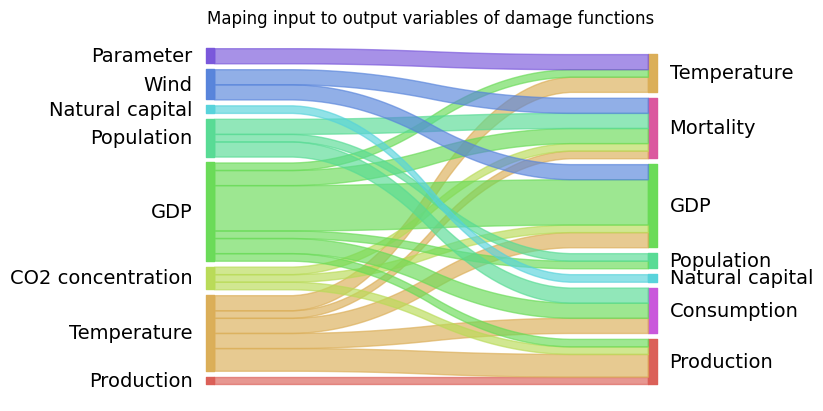
\includegraphics[width=0.9\linewidth]{figures/sankey.png}
    \legende{Sankey diagram des différentes fonctions}{Les modèles ne prennent pas en compte tous les mêmes données en entrées, et elles ne permettent pas d'expliquer les mêmes phénomènes. Production par les auteurs.}
    \label{fig:sankey}
\end{figure}

\subsection{La calibration : un \textit{"tiens"} vaut-il deux \textit{"tu l'auras"} ?}

\section{Trois querelles pour répondre à ces questions}

\subsection{Le taux d'actualisation : la querelle Nordhaus / Stern}

La controverse qui oppose William Nordhaus et Nicolas Stern est un exemple classique des enjeux éthiques et normatifs induit par la modélisation intégrée. Il est bien expliquée dans \cite{guigourez_10_2023}, sur lequel on va s'appuyer pour rappeler ici les enjeux de cette querelle. \\

William Nordhaus est un économiste des Etats-Unis. Au début des années 1990, il met au point le modèle DICE, qui est une des premiers à modéliser l'interaction climat - économie. Ce modèle sera ensuite mis à jour régulièrement, et sera suivi de RICE, un modèle plus régionalisé. Il obtient le Prix dit Nobel d'Economie en 2018 pour ses l'intégration du changement climatique dans l'analyse macro-économique que long terme\cite{yale}. Adepte de la théorie des choix publics, il pense que l'inaction climatique vient d'une mauvaise appréciation des coûts futurs du changement climatique, et qu'une analyse coût-bénéfice permet de suivre des trajectoires climatiques plus optimales. 
Sir Nicolas Stern a été vice-président senior de la Banque Mondiale de 2000 à 2003. Peu après, le gouvernement britannique lui commande un rapport sur les effets du changement climatique sur l'économie. \\

Les deux auteurs utilisent des modèles intégrés : Nordhaus utilise DICE, et Stern utilise PAGE. Les deux modèles sont similaires en termes d'hypothèses et de fonctionnement. Ces modèles sont des modèles d'optimisation, qui visent à donner un coût optimal à une tonne de carbone. Ils sont d'ailleurs utilisés pour calculer le coût social du carbone (voir figure \ref{fig:scc}). Pour pouvoir comparer le coût de politiques publiques aujourd'hui, aux gains ultérieurs (c'est-à-dire aux dommages futurs évités), il faut pouvoir comparer ces deux grandeurs. \\

Cependant, on considère que la valeur de l'argent dans le futur est plus faible qu'aujourd'hui. De nombreux facteurs permettent d'arriver à cette conclusion : le futur est incertain, et il est donc possible que ces événements ne se réalisent pas; ou alors que les générations futures soient capable de mieux y faire face; ou tout simplement, nous préférons nos générations aux générations ultérieures. C'est une formalisation de l'adage : \emph{un tiens vaut deux tu l'auras}. La question est donc de savoir \emph{à quel point} les dommages futurs sont moins importants que ceux d'aujourd'hui, ou encore combien de \emph{tu l'auras} un \emph{tiens} vaut-il ? \\

Formellement, on retient la structure suivante : 

\begin{equation}
    r_t = \delta + \eta g_t 
    \label{eq:disc_rate}
\end{equation}

où $r_t$ représente le taux d'actualisation de la consommation à l'instant $t$, $\delta$ représente la préférence pure pour le présent, $\eta$ l'élasticité marginale de l'utilité en fonction de la consommation, c'est-à-dire à quel point les agents peuvent adapter leurs préférences,  et $g_t$ le taux de croissance de la consommation. \\

Cette formulation permet d'intégrer la préférence pure pour le présent, appelée aussi taux d'actualisation de l'utilité, dans la fonction de consommation. C'est ainsi qu'elle est implémentée dans DICE et PAGE. À partir d'ici, nous nous intéresserons uniquement à $\delta$, que nous appellerons taux d'actualisation. \\

Nordhaus utilise comme paramètres $\delta = 1.5\%$ et $\eta=2$, tandis que Stern utilise $\delta=0.1\%$ et $\eta=1$. Ainsi, Stern considère que l'on doit prendre en compte les dommages causés aux générations futures (presque) comme s'ils survenaient maintenant; tandis que Nordhaus considère qu'il faut les prendre en compte en retirant 1,5\% de leur valeur chaque année. \\

À partir de ces simples hypothèses, et en utilisant des similaires, les auteurs obtiennent des résultats drastiquement différents. Stern suggère des investissements massifs et rapides, tandis que Nordhaus promeut de faibles investissements aujourd'hui, pour n'investir que plus tard. 

\cite{guigourez_10_2023} => description de la querelle

\begin{figure}
    \centering
    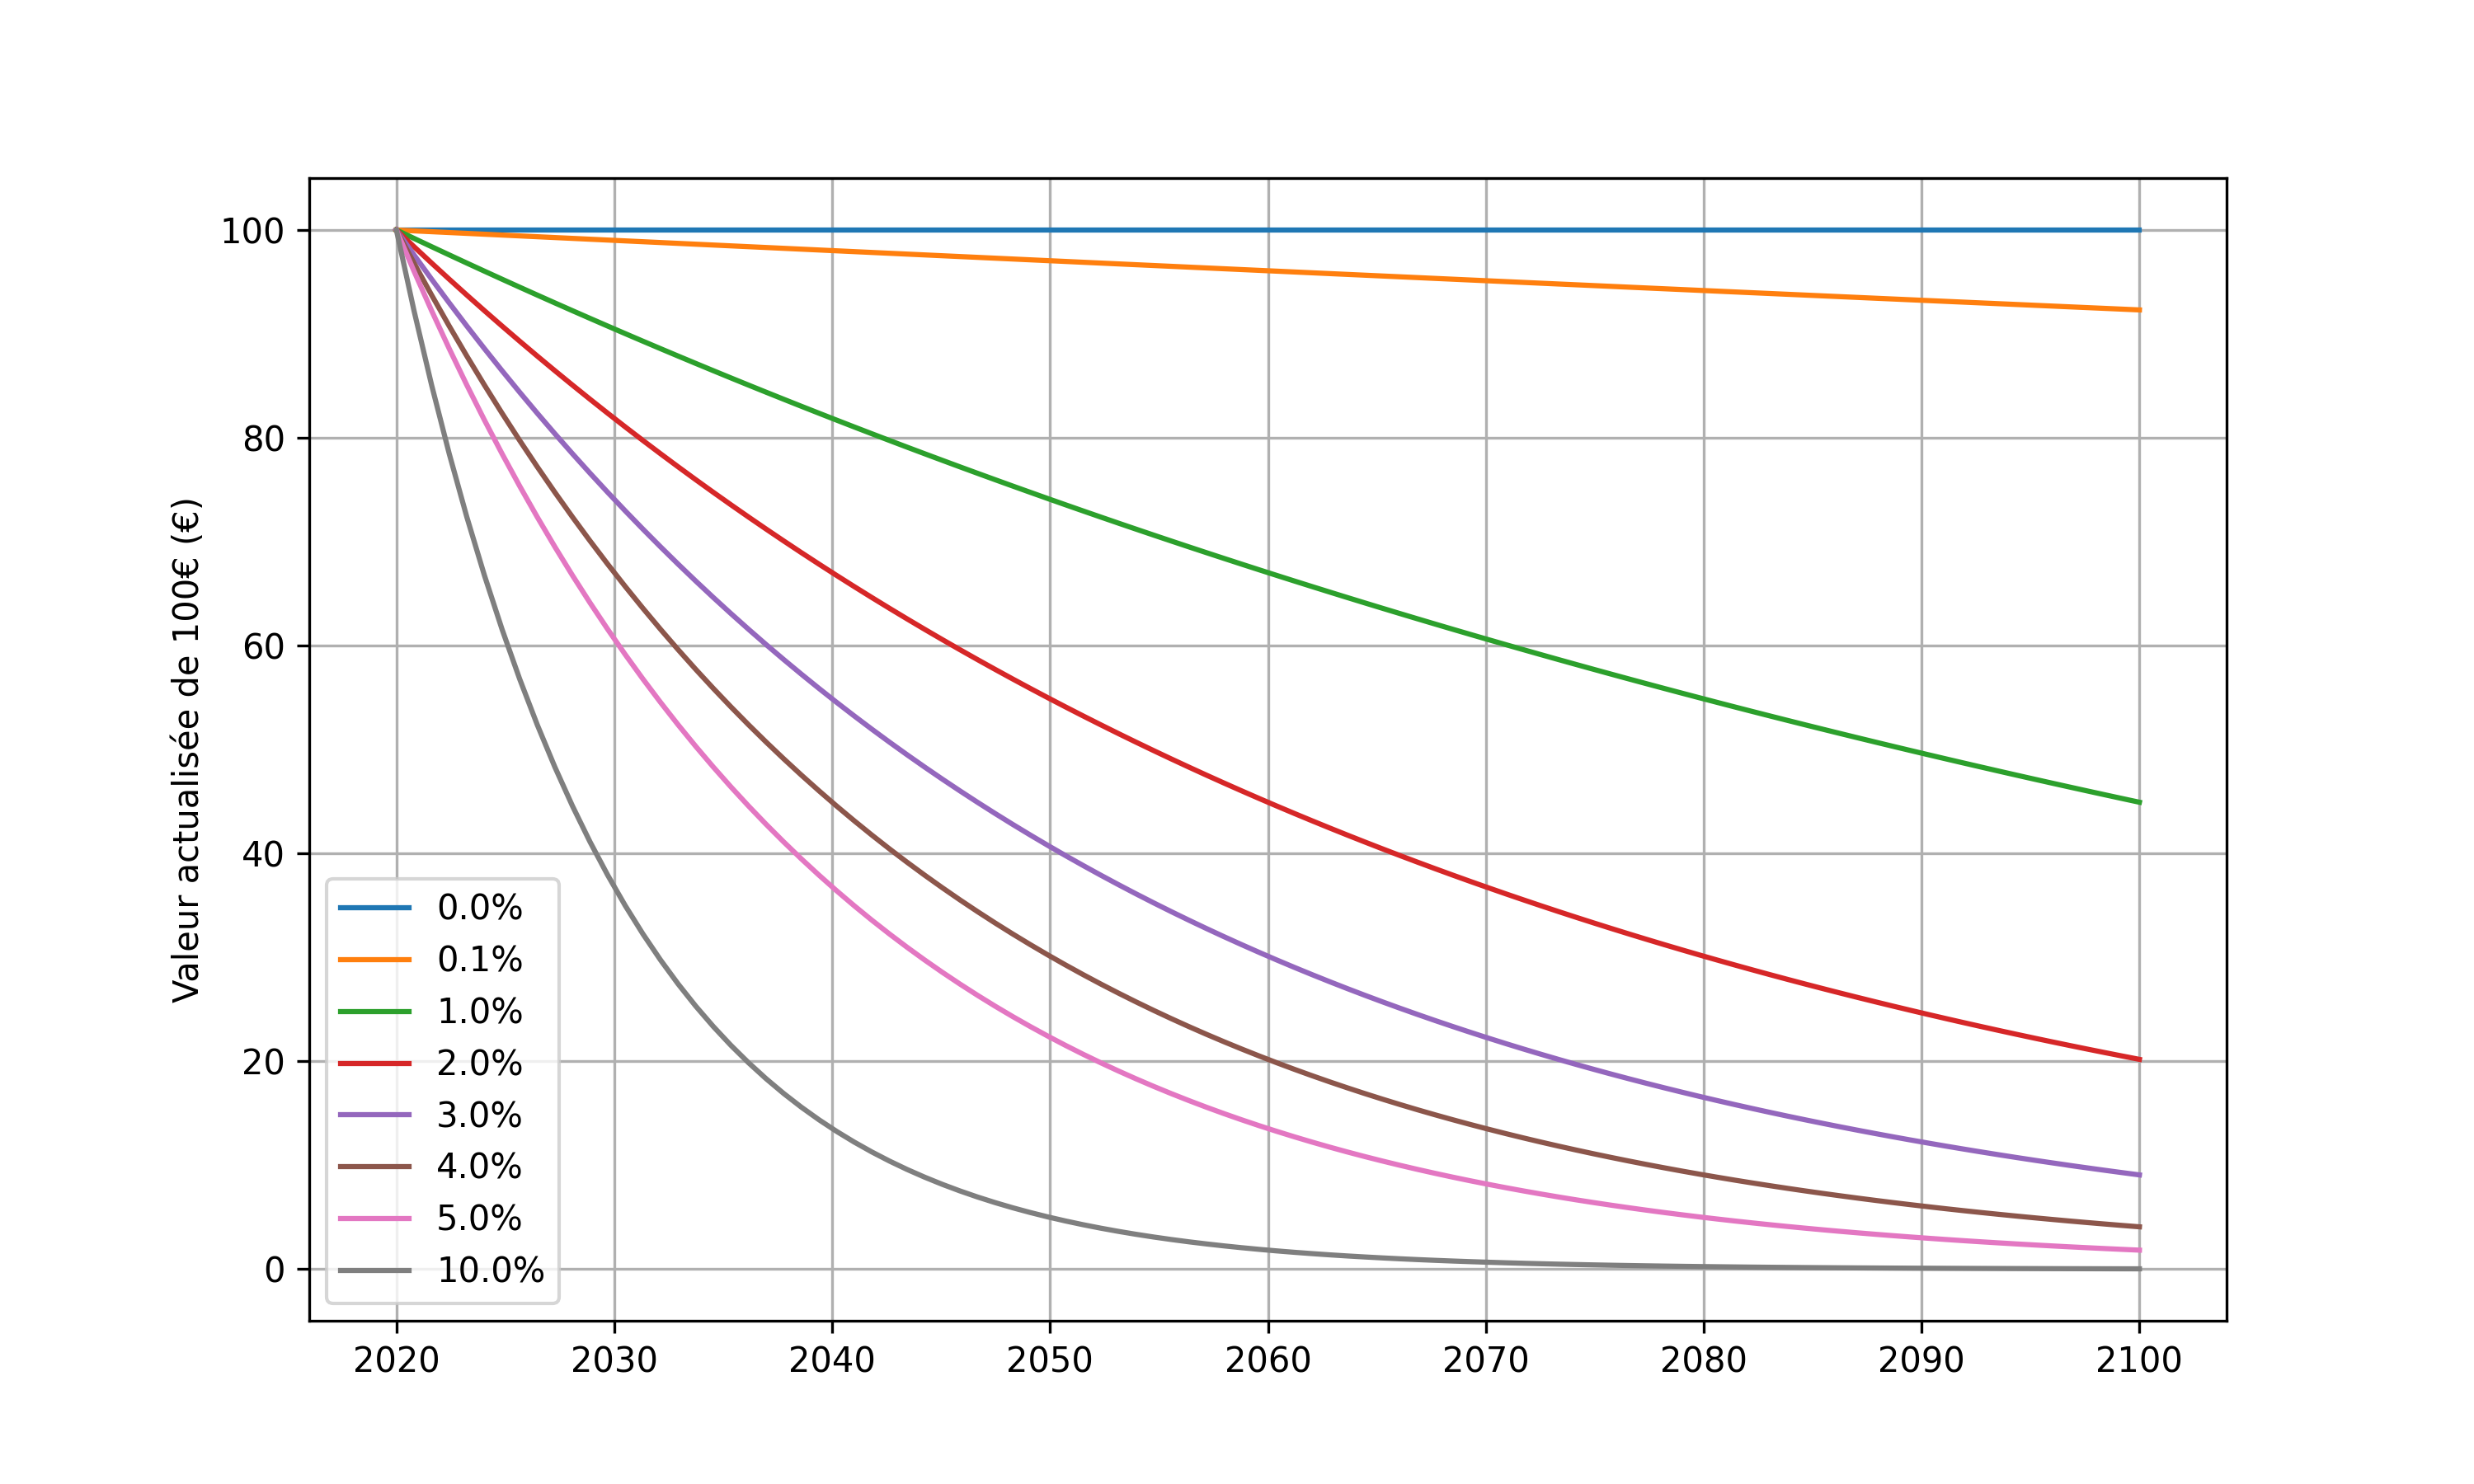
\includegraphics[width=\linewidth]{results/actualisation.png}
    \legende{Valeur actualisée selon le temps et le taux d'actualisation}{Graphique qui représente la valeur d'une unité monétaire dans le temps, actualisée au présent, selon le taux d'actualisation. En jaune, celui choisi par Nordhaus, et en bleu celui choisi par Stern. Clé de lecture : avec un taux d'actualisation de 3\%, 100\$ de dommage en 2080 ne valent que 18\$ en 2020, alors que 100\$ de 2040 valent 56\$. }
    \label{fig:discount-rate}
\end{figure}

\subsection{Pourquoi représenter les dommages ? Les SCC vs le reste du monde}

Comme nous avons pu le voir, les critiques quant à la quantification et la monétarisation des dommages sont déjà nombreuses. Se pose donc la question suivante : faut-il représenter les dommages, et si oui, pourquoi et comment ? Pour éclairer ce dilemne, nous allons nous pencher sur deux une distinction particulière, entre les modèles qui représentent les dommages et ceux qui ne le font pas. \\

D'une part, certains modèles représentent des dommages de manière explicite. Ce sont essentiellement des modèles utilisés pour mesurer le coût social du carbone. Les arguments qui sont avancés par leurs défenseurs sont solides. Nous vivons dans un monde où la valorisation économique est centrale. Conformément à la théorie économique, et notamment à celle consacrée aux biens communs et aux externalités, si on ne peut pas compter la valeur de quelque chose, et surtout qu'elle ne s'impose pas à nous lors des transactions, alors cette valeur est invisible. De ce point de vue, et malgré les nombreuses limites (souvent assumées d'ailleurs) de la modélisation de ces phénomènes, il est nécessaire de représenter les dommages dans le modèle, même de manière imparfaite. En effet, selon ce point de vue, ne pas les représenter revient à les négliger, les omettre, ou en d'autre terme, à leur attribuer arbitrairement une valeur nulle. 
C'est dans cette perspective que se place de nombreux modèles, qui cherchent à proposer de nouvelles manières de représenter les dommages. Nombreux sont ceux qui, en réponse à la simplicité de la représentation de Nordhaus, ont proposé des fonctions de dommage toujours plus complexe, prenant en compte plus de mécanismes. 
\\

D'autre part, on peut argumenter que la représentation de ces dommages donne une fausse sensation de certitude. D'une part, elle done l'impression que le modèle est plus réaliste, en ce sens que ce qu'il dit \textit{serait} plus proche de la réalité et moins sujet aux travers de la simplification car justement plus complexe. Pourtant, on peut argumenter que la représentation des dommages, y compris quand elle est sophistiquée, fait appel à de nombreuses hypothèses, notamment concernant la permanence des phénomènes qui ont lieu. On a alors un modèle qui non seulement n'est pas forcément plus fiable ou plus proche de la réalité, mais qui est en plus nettement moins lisible, compréhensible - et dont les limites ne peuvent que très difficilement être interprétées et critiquées. 

\subsection{Compter ce qui n'a pas de prix : la difficile monétarisation}



\begin{figure}
    \centering
    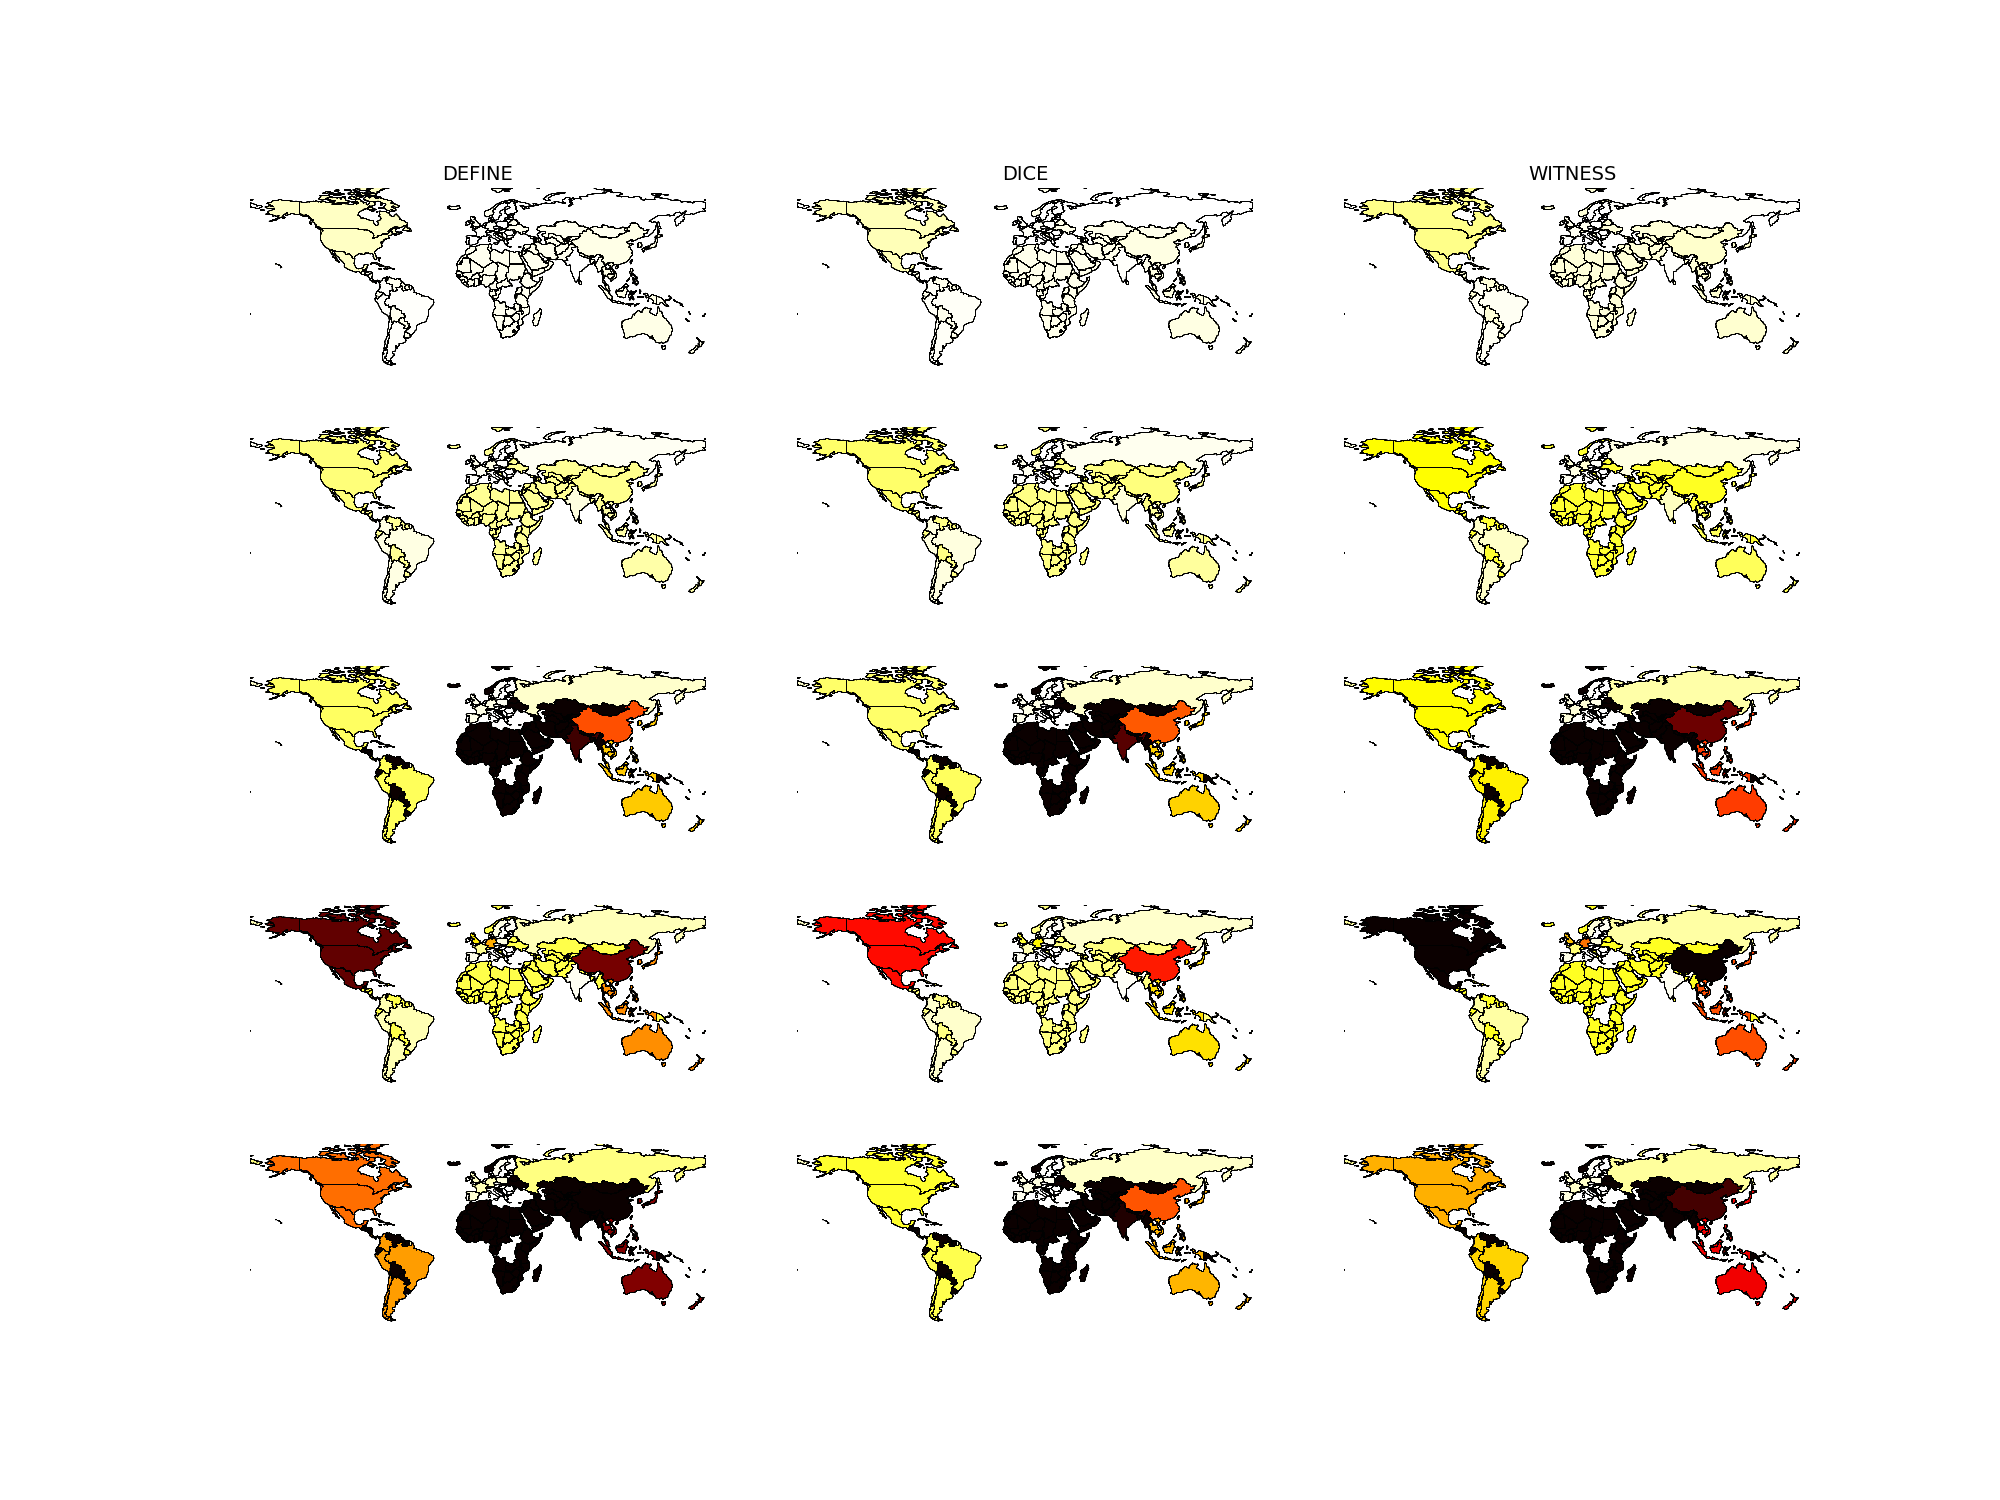
\includegraphics[width=\linewidth]{results/carte_progressive.png}
    \legende{Double progression du niveau de dommage}{Le niveau de dommage suit une double progression. D'une part, il augmente avec le temps (qui est lui même très lié au niveau de réchauffement); d'autre part, il augmente avec le modèle : certains modèles donnent des niveaux de dommage plus importants que d'autres.}
    \label{fig:carte-progressive}
\end{figure}
TODO 


